% !TEX encoding = UTF-8 Unicode
\documentclass[a4paper]{article}
\usepackage{color}
\usepackage{url}
\usepackage{listings}
\usepackage[T2A]{fontenc} % enable Cyrillic fonts
\usepackage[utf8]{inputenc} % make weird characters work
\usepackage{graphicx}
\usepackage{setspace} 
\usepackage{graphics}

\usepackage[english,serbian]{babel}
%\usepackage[english,serbianc]{babel} %ukljuciti babel sa ovim opcijama, umesto gornjim, ukoliko se koristi cirilica

\usepackage[unicode]{hyperref}
\hypersetup{colorlinks,citecolor=green,filecolor=green,linkcolor=blue,urlcolor=blue}
\usepackage{float}

%\newtheorem{primer}{Пример}[section] %ćirilični primer
\newtheorem{primer}{Primer}[section]

\definecolor{mygreen}{rgb}{0,0.6,0}
\definecolor{mygray}{rgb}{0.5,0.5,0.5}
\definecolor{mymauve}{rgb}{0.58,0,0.82}

\lstset{ 
  backgroundcolor=\color{white},   % choose the background color; you must add \usepackage{color} or \usepackage{xcolor}; should come as last argument
  basicstyle=\scriptsize\ttfamily,        % the size of the fonts that are used for the code
  breakatwhitespace=false,         % sets if automatic breaks should only happen at whitespace
  breaklines=true,                 % sets automatic line breaking
  captionpos=b,                    % sets the caption-position to bottom
  commentstyle=\color{mygreen},    % comment style
  deletekeywords={...},            % if you want to delete keywords from the given language
  escapeinside={\%*}{*)},          % if you want to add LaTeX within your code
  extendedchars=true,              % lets you use non-ASCII characters; for 8-bits encodings only, does not work with UTF-8
  firstnumber=1000,                % start line enumeration with line 1000
  frame=single,	                   % adds a frame around the code
  keepspaces=true,                 % keeps spaces in text, useful for keeping indentation of code (possibly needs columns=flexible)
  keywordstyle=\color{blue},       % keyword style
  language=Python,                 % the language of the code
  morekeywords={*,...},            % if you want to add more keywords to the set
  numbers=left,                    % where to put the line-numbers; possible values are (none, left, right)
  numbersep=5pt,                   % how far the line-numbers are from the code
  numberstyle=\tiny\color{mygray}, % the style that is used for the line-numbers
  rulecolor=\color{black},         % if not set, the frame-color may be changed on line-breaks within not-black text (e.g. comments (green here))
  showspaces=false,                % show spaces everywhere adding particular underscores; it overrides 'showstringspaces'
  showstringspaces=false,          % underline spaces within strings only
  showtabs=false,                  % show tabs within strings adding particular underscores
  stepnumber=2,                    % the step between two line-numbers. If it's 1, each line will be numbered
  stringstyle=\color{mymauve},     % string literal style
  tabsize=2,	                   % sets default tabsize to 2 spaces
  title=\lstname                   % show the filename of files included with \lstinputlisting; also try caption instead of title
}


\begin{document}
\title{Izveštaj primene alata za verifikaciju u okviru samostalnog praktičnog projekta na kursu Verifikacija Softvera
\\\small{ Matematički fakultet}}
\author{Nikola Mićić, 1086/2022 \\
\normalsize {nikolamicic065@gmail.com} \\ 
\normalsize {Mentor: Ivan Ristović}
}

\date{Decembar  2022.}

\maketitle
\abstract{
Ovaj rad će sadržati detaljan opis analize projekta sa spiskom naredbi i alata koji su korišćene i zaključcima koji su napravljeni.

Projekat nad kojim će biti primenjeni alati se nalazi na github adresi: https://github.com/eminfedar/widgetci

Autor ovog projekta je Emin Fedar (github username: eminfedar).

Primena alata će biti izvršena na master grani, nad komitom čiji je hash code sledeći: 05588c036cd4c6d6eddd5b595d027968ac484140
}


\begin{spacing}{0.7}
    \tableofcontents
\end{spacing}

\newpage
\section{Spisak primenjenih alata}
Spisak alata za verifikaciju koji su primenjeni nad projektom su:

\begin{enumerate}
    \item Clang-tidy i Clazy
\end{enumerate}

\subsection{Clang-tidy i Clazy}
Clang-tidy pruža dijagnostiku i ispravke za tipične programske greške, kao što su kršenje stila ili zloupotreba interfejsa.

Clazy pomaže Clang-u da razume Qt semantiku. Prikazuje upozorenja kompajlera vezana za Qt, u rasponu od nepotrebne alokacije memorije do zloupotrebe API-ja i pruža akcije refaktorisanja za rešavanje nekih problema.

Clang-tidy i Clazy su alati koji su pokrenuti preko QtCreator-a.
Alat je pokrenut preko Debug moda i sastoji se iz narednih koraka koji se mogu videti na slikama ispod.

Prvi korak je biranje alata Clang-Tidy i Clazy u okviru padajućeg menija Analyze.

\begin{figure}[h!]
\begin{center}
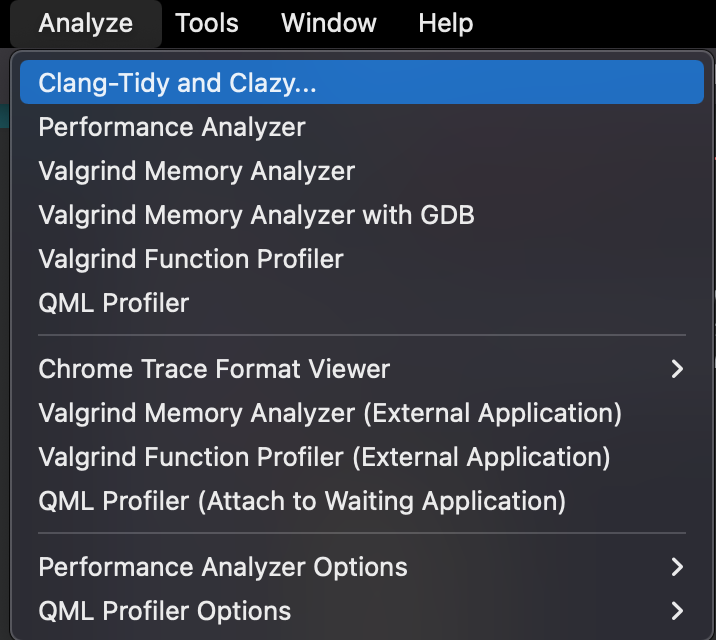
\includegraphics[scale=0.45]{clang-tidy-01.png}
\end{center}
\caption{Prvi korak}
\label{fig: clang-tidy-0}
\end{figure}

Drugi korak se sastoji iz biranja fajlova koji će biti analizirani. U ovom slučaju sam birao sve fajlove uključujući glavni folder \textit{code} u okviru kojeg se nalaze podfolderi \textit{headers} i \textit{src}. Nakon toga kliknuti dugme \textit{Analyze}.

\begin{figure}[h!]
\begin{center}
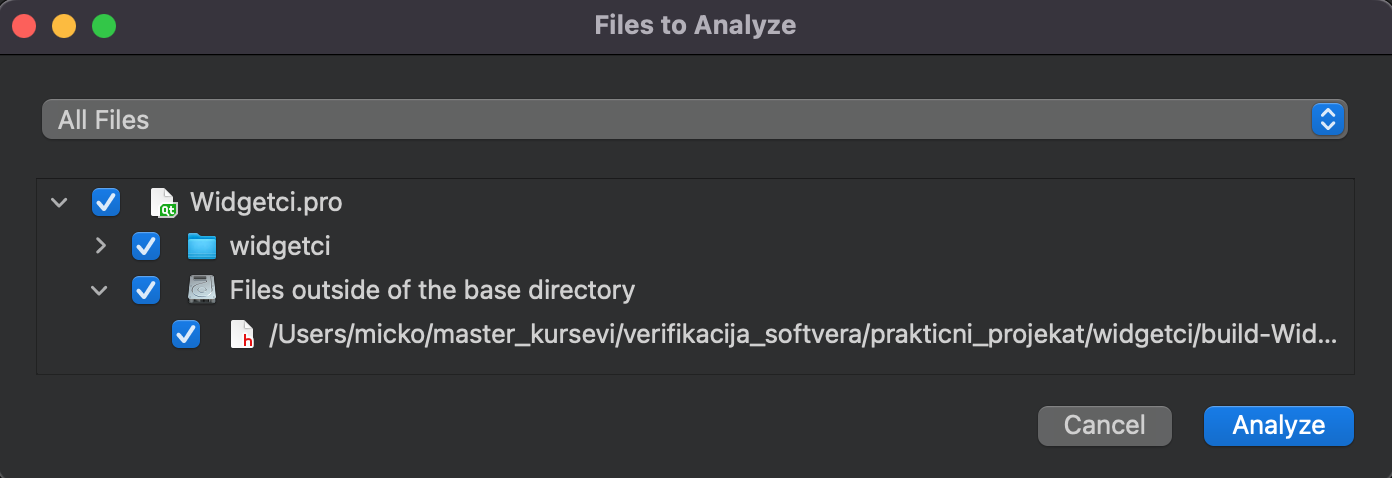
\includegraphics[scale=0.35]{clang-tidy-02.png}
\end{center}
\caption{Drugi korak}
\label{fig: clang-tidy-2}
\end{figure}

\newpage
Deo rezultata ovih alata je predstavljen na slici \ref{fig: clang-tidy-3} ispod. Može se videti upozorenje da postoji neinicijalizovano polje na kraju poziva konstruktora, sa objašnjenjima. 
Ceo izlaz pozvanih alata se može naći u okviru repozitorijuma za analizu datog projekta, u okviru foldera Clang-tidy i Clazy.

\begin{figure}[h!]
\begin{center}
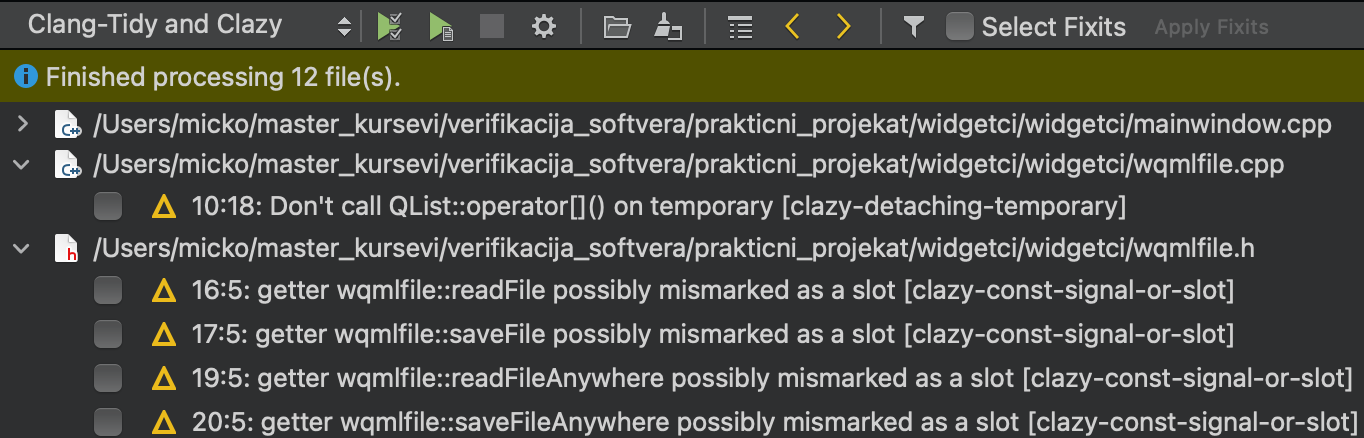
\includegraphics[scale=0.45]{clang-tidy-03.png}
\end{center}
\caption{Deo rezultata pozvanih alata}
\label{fig: clang-tidy-3}
\end{figure}

\subsection{Cppcheck}
Cppcheck je alat za statičku analizu za C/C++ kod. Pruža jedinstvenu analizu koda za otkrivanje grešaka i fokusira se na otkrivanje nedefinisanog ponašanja i opasnih konstrukcija kodiranja. Cilj je imati vrlo malo lažnih pozitivnih rezultata. Cppcheck je dizajniran da može da analizira vaš C/C++ kod čak i ako ima nestandardnu sintaksu (uobičajeno u ugrađenim projektima).

Cppcheck je alat koji sam pokretao preko terminala. Za instalaciju alata na macOS-u sam koristio komandu \textit{brew install cppcheck}.

Alat proverava sve .cpp fajlove na prosleđenoj putanji i vraća uočene greške i upozorenja.

Pozivanje komande i deo rezultata je izgledao kao na slici ispod.

Greška koja je otkrivena na slici \ref{fig: cppcheck-0} je pronađena u fajlu widgetci/wqmlsystem.cpp na liniji 78 i predstavlja pronađenu funkciju koja je non-void tipa, a ipak ne sadrži povratnu vrednost.

Celokupan izlaz pozivanja alata se može naći u okviru repozitorijuma za analizu datog projekta, u okviru foldera Cppcheck.

\begin{figure}[h!]
\begin{center}
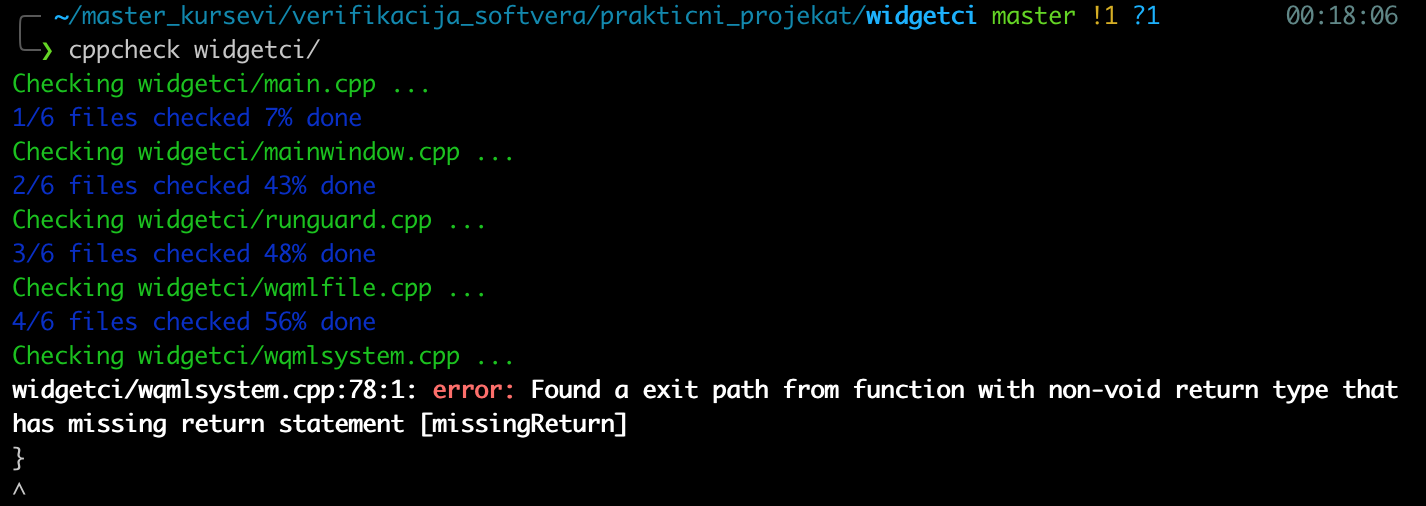
\includegraphics[scale=0.45]{cppcheck-00.png}
\end{center}
\caption{Način pokretanja i rezultati alata cppcheck}
\label{fig: cppcheck-0}
\end{figure}

\subsection{GCov}

GCov je alat za analizu pokrivenosti izvornog koda i alat za profilisanje izraz-po-izraz. Gcov generiše tačne brojeve koliko puta je svaki izraz u programu izvršen. Gcov dolazi kao standardni uslužni program sa GNU Compiler Collection (GCC) paketom.

Primena alata GCov je urađena iz sledećih koraka.
Prvo su u \textit{Widgetci.pro} fajlu dodata dva flega:

\begin{itemsize}
    \item \texttt{QMAKE\_CXXFLAGS += --coverage}
    \item \texttt{QMAKE\_LFLAGS += --coverage}
\end{itemsize}

Izgradnja projekta sa novim flagovima je generisala naredne fajlove, među kojima su i dodatno generisani fajlovi koji imaju ekstenziju '.gcno' i '.gcda'. Svi fajlovi se mogu videti na slici 
\ref{fig: GCov-00}

\begin{figure}[h!]
\begin{center}
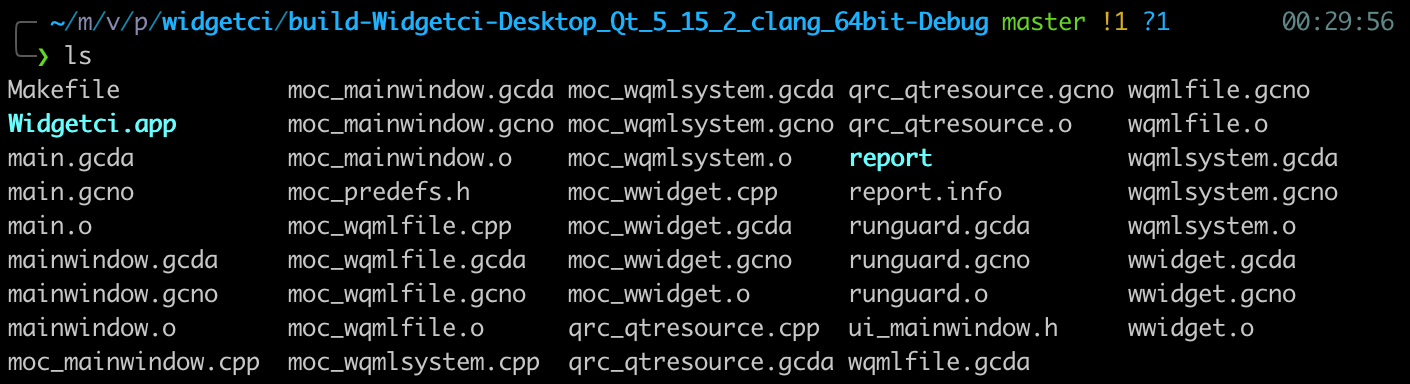
\includegraphics[scale=0.45]{GCov-00.png}
\end{center}
\caption{Generisani fajlovi}
\label{fig: GCov-00}
\end{figure}

Zatim je pokrenuta naredba koja kreira traženi izveštaj u datoteci \textit{report.info}, a rezultat naredbe možemo videti na sledećoj slici \ref{fig: GCov-01}

\begin{figure}[h!]
\begin{center}
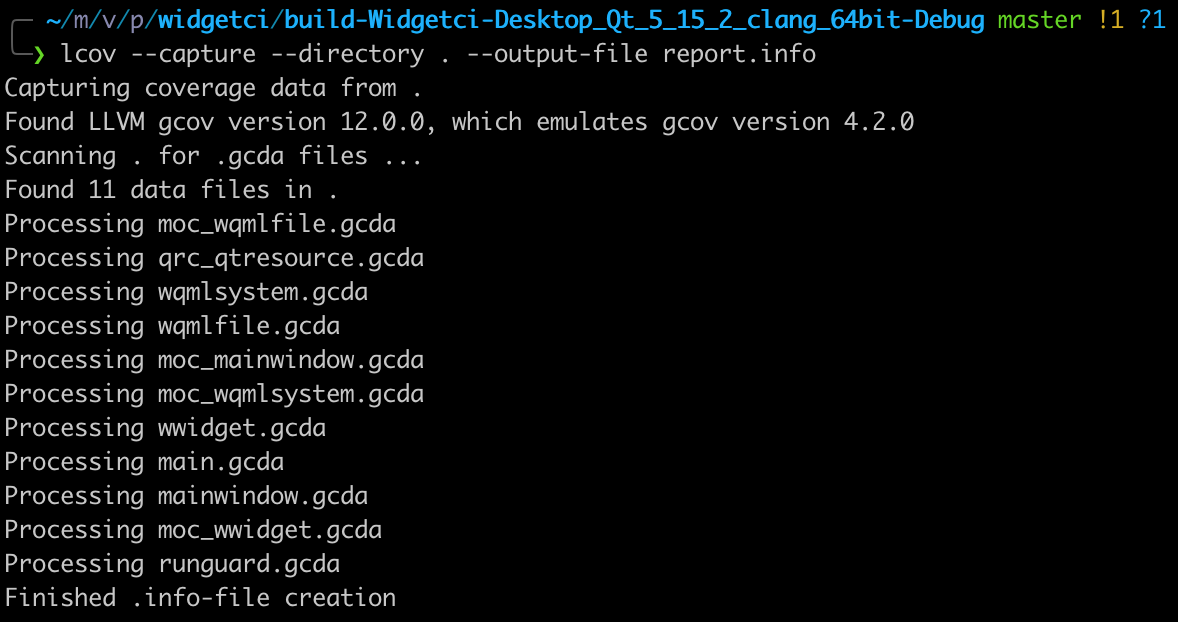
\includegraphics[scale=0.45]{GCov-01.png}
\end{center}
\caption{rezultat poziva lcov naredbe}
\label{fig: GCov-01}
\end{figure}

Komandom \textbf{genhtml -o report report.info} dobijamo html izveštaj preko podataka iz \textit{report.info} datoteke, a kompletni izlazi prethodne dve komande se mogu naći u okviru repozitorijuma za analizu datog projekta, u okviru foldera GCov.

U folderu report unutar build foldera se nalazi ceo izveštaj, a html verziju izveštaja možemo videti otvaranjem index.html fajla i ona izgleda kao na slici \ref{fig: GCov-02} ispod.

\begin{figure}[h!]
\begin{center}
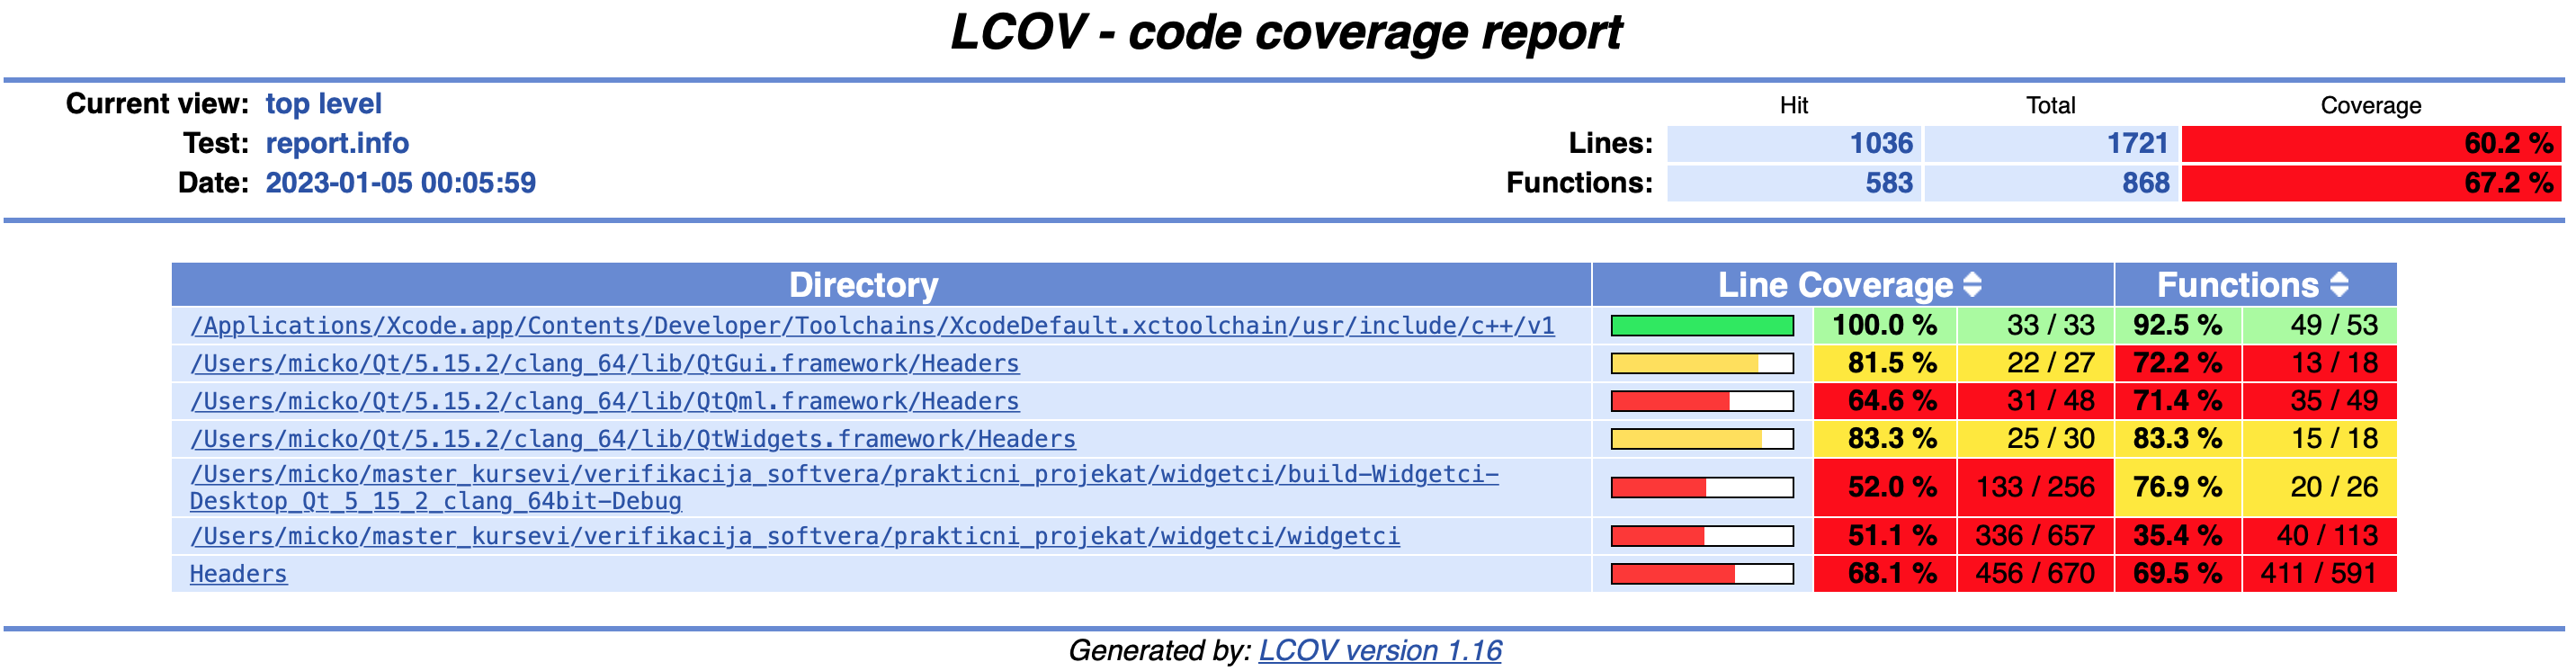
\includegraphics[scale=0.23]{GCov-02.png}
\end{center}
\caption{html verzija izveštaja pokrivenosti koda}
\label{fig: GCov-02}
\end{figure}

Detaljniji prikaz pokrivenosti koda nad fajlovima u okviru projekta možemo videti klikom na neki od ponuđenih putanja. Klikom na folder i podfolder \textit{widgetci}, otvara se analiza pokrivenosti koda izlistanih fajlova koji se mogu videti na slici \ref{fig: GCov-03} ispod.

\begin{figure}[h!]
\begin{center}
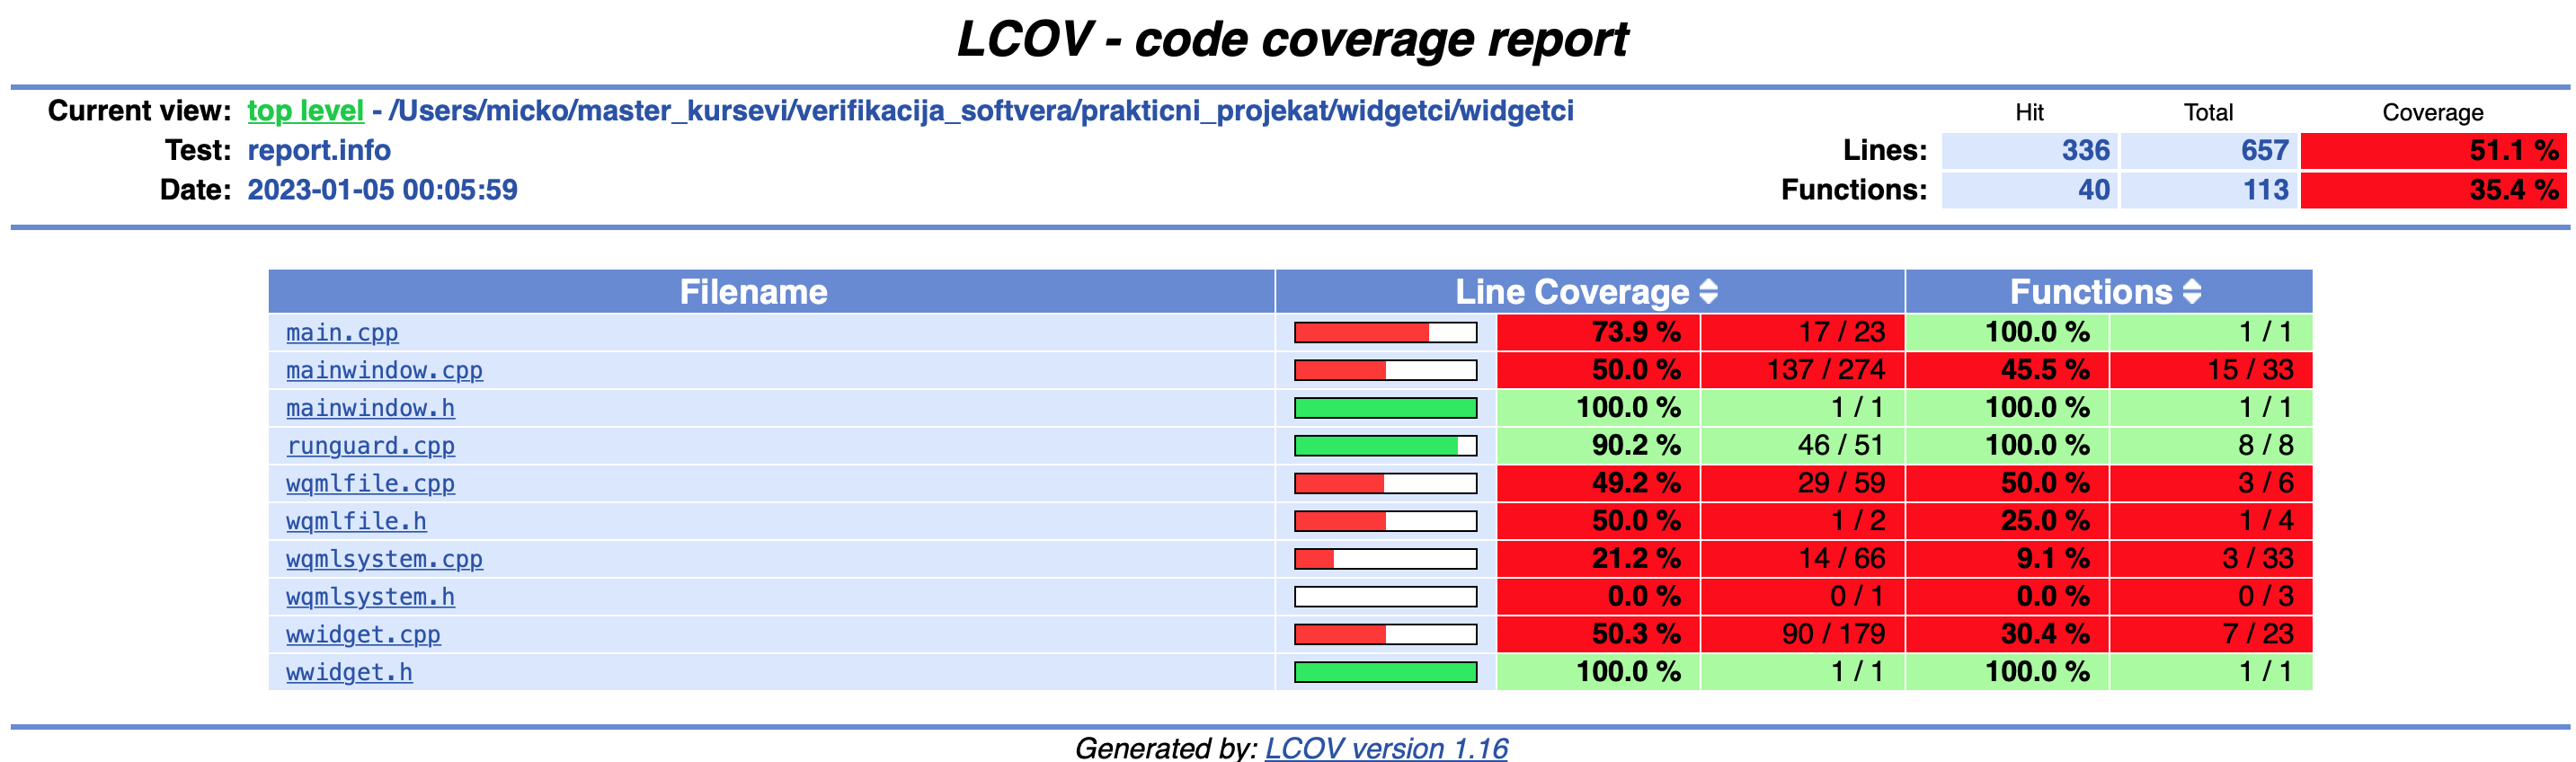
\includegraphics[scale=0.23]{GCov-03.png}
\end{center}
\caption{detaljniji prikaz izveštaja pokrivenosti koda}
\label{fig: GCov-03}
\end{figure}

\subsection{QML Profiler}
QML Profiler je alat koji omogućava da se dobiju neophodne dijagnostičke informacije, omogućujuću da se analizira kod aplikacije kako bi se otkrili problemi sa performansama. Primer problema sa performansama predstavljaju previše JavaScript-a u određenim frejmovima, C++ funkcija koje traju predugo ili troše previše memorije.
QML Profiler predstalvja deo i Qt Creator-a i Qt Design Studio-a.

Kroz korake će biti predstavljen način rada ovog alata i rezultati prikazani.

Pokretanje alata preko Qt Creator-a se vrši preko padajućeg menija Analyze i biranje alata QML Profiler, kao na slici \ref{fig: qml-00} ispod.

\begin{figure}[h!]
\begin{center}
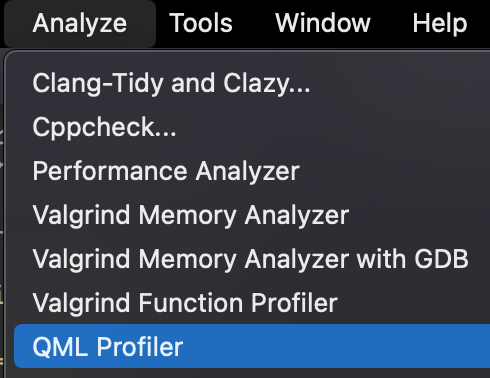
\includegraphics[scale=0.45]{qml-prof-00.png}
\end{center}
\caption{Biranje alata QML Profiler-a}
\label{fig: qml-00}
\end{figure}


Zatim se na zeleno dugme pokreće alat, kao što se može videti na slici \ref{fig: qml-01} ispod.

\begin{figure}[h!]
\begin{center}
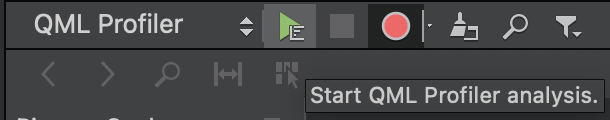
\includegraphics[scale=0.45]{qml-prof-01.png}
\end{center}
\caption{Pokretanje QML Profiler-a}
\label{fig: qml-01}
\end{figure}

Analiza QML Profiler-a je odrađena pri pokretanju widget-a aplikacije koja predstavlja prikazivanje slike sata koja može da se povećava i smanjuje pomeranjem donje desne ivice kao što se može videti na slici \ref{fig: qml-02} ispod.

\begin{figure}[h!]
\begin{center}
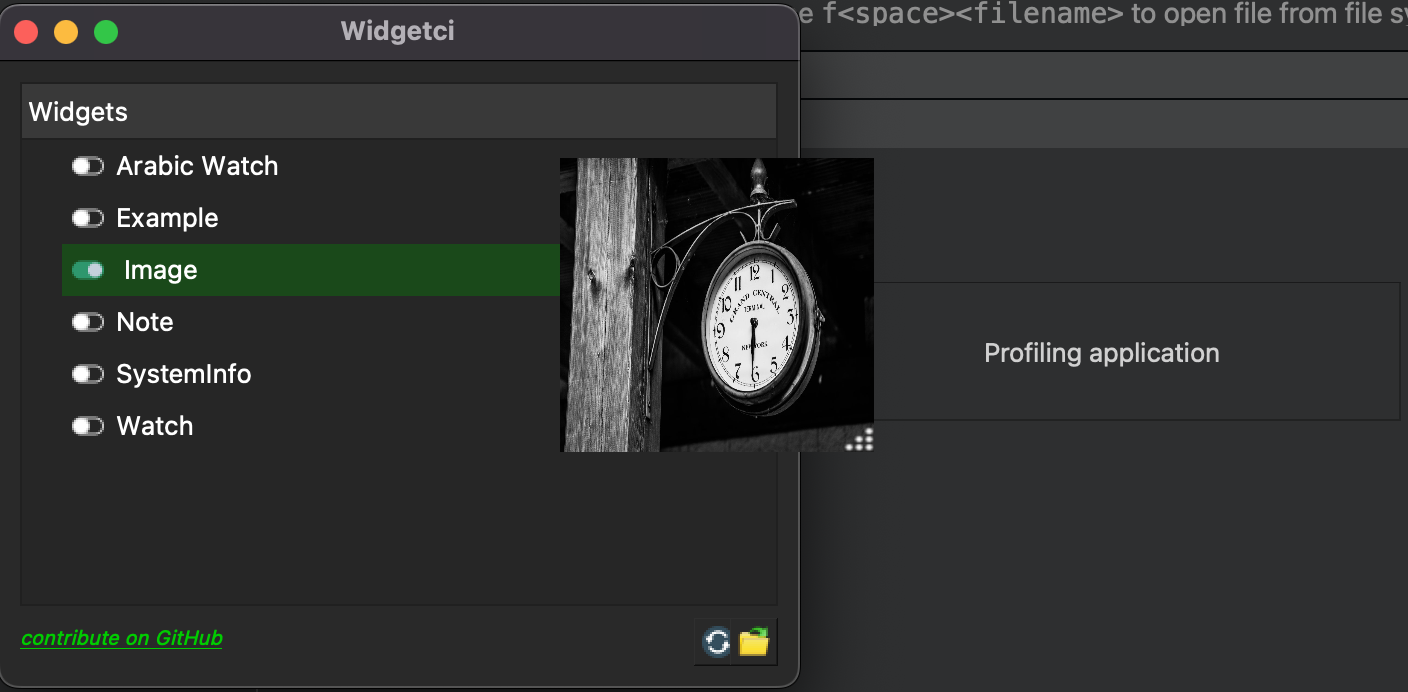
\includegraphics[scale=0.40]{qml-prof-02.png}
\end{center}
\caption{Interakcija sa aplikacijom tokom analiziranja QML Profiler-om}
\label{fig: qml-02}
\end{figure}

Rezultati QML Profiler-a predstavljaju analizu nakon 10 sekundi prikazivanja sata i povećavanja i smanjivanja njegovih dimenzija pomeranjem donje desne ivice.

Timeline QML Profiler-a izdeljen po sekcijama u prvoj sekundi izvršavanja izgleda kao na slikama \ref{fig: qml-03},\ref{fig: qml-04}  (duže od jedne sekunde nije moglo biti prikazano na screenshot-u)

\begin{figure}[h!]
\begin{center}
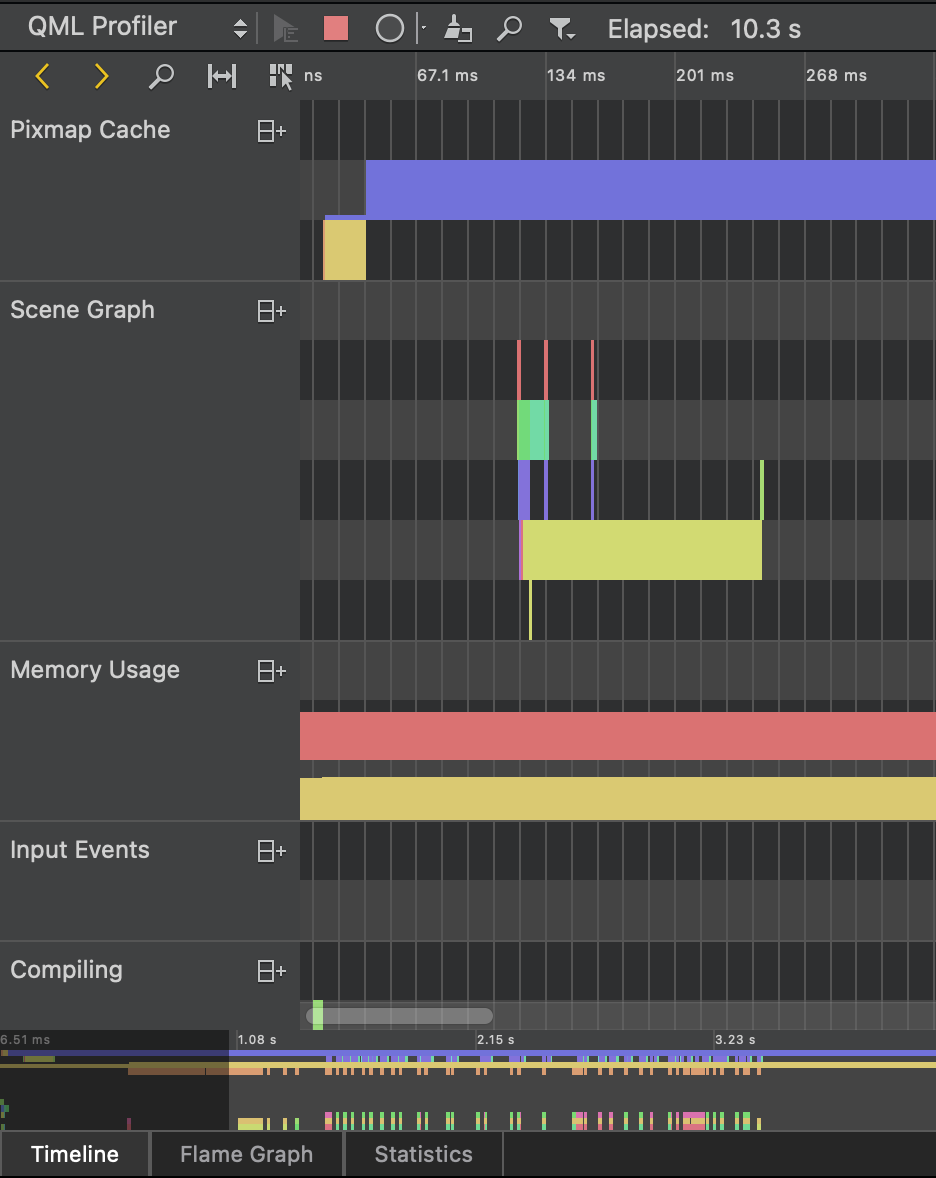
\includegraphics[scale=0.40]{qml-prof-03.png}
\end{center}
\caption{Prvi deo Timeline-a QML Profiler-a}
\label{fig: qml-03}
\end{figure}

\begin{figure}[h!]
\begin{center}
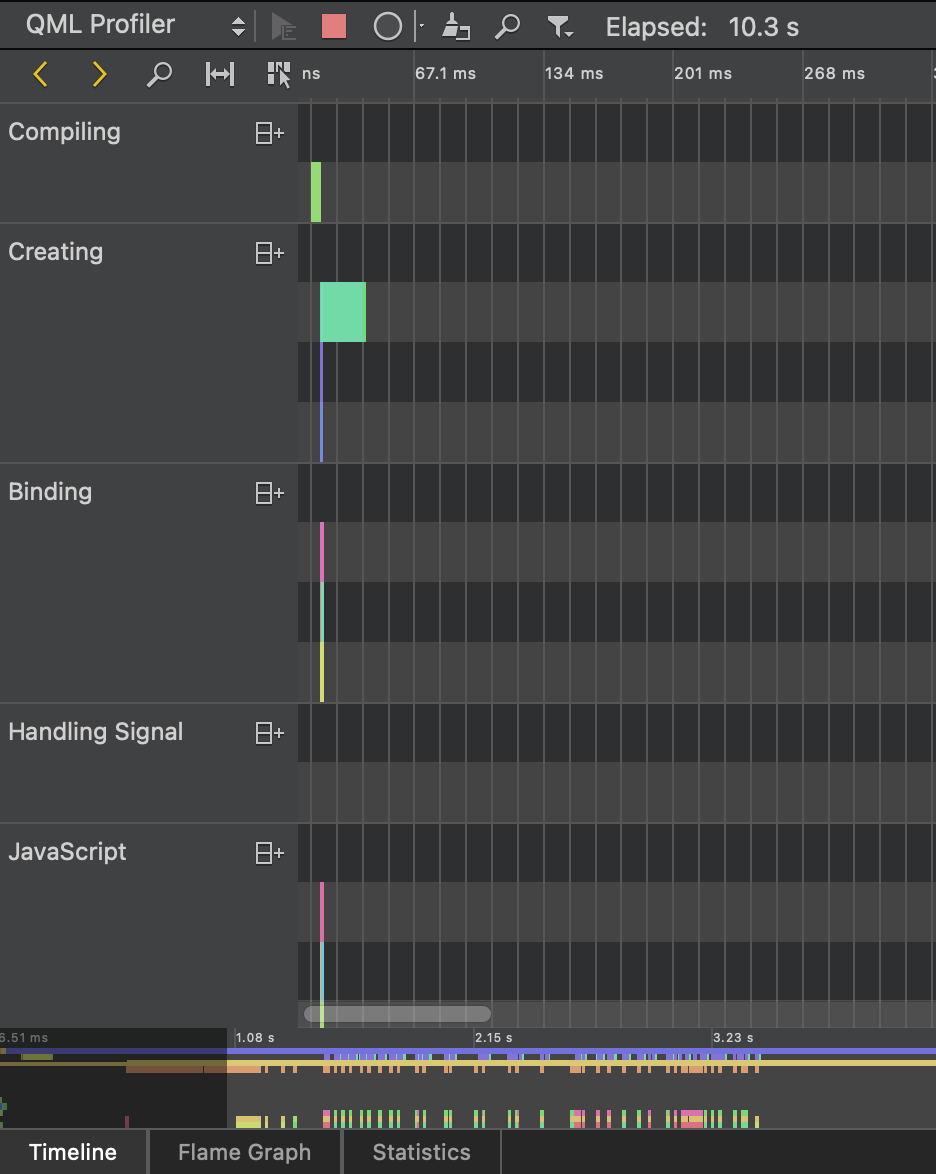
\includegraphics[scale=0.40]{qml-prof-04.png}
\end{center}
\caption{Drugi deo Timeline-a QML Profiler-a}
\label{fig: qml-04}
\end{figure}

\newpage
Rezultat analize prikazan kroz Flame Graph, za sekciju Total Time izgleda ovako \ref{fig: qml-05}.

\begin{figure}[h!]
\begin{center}
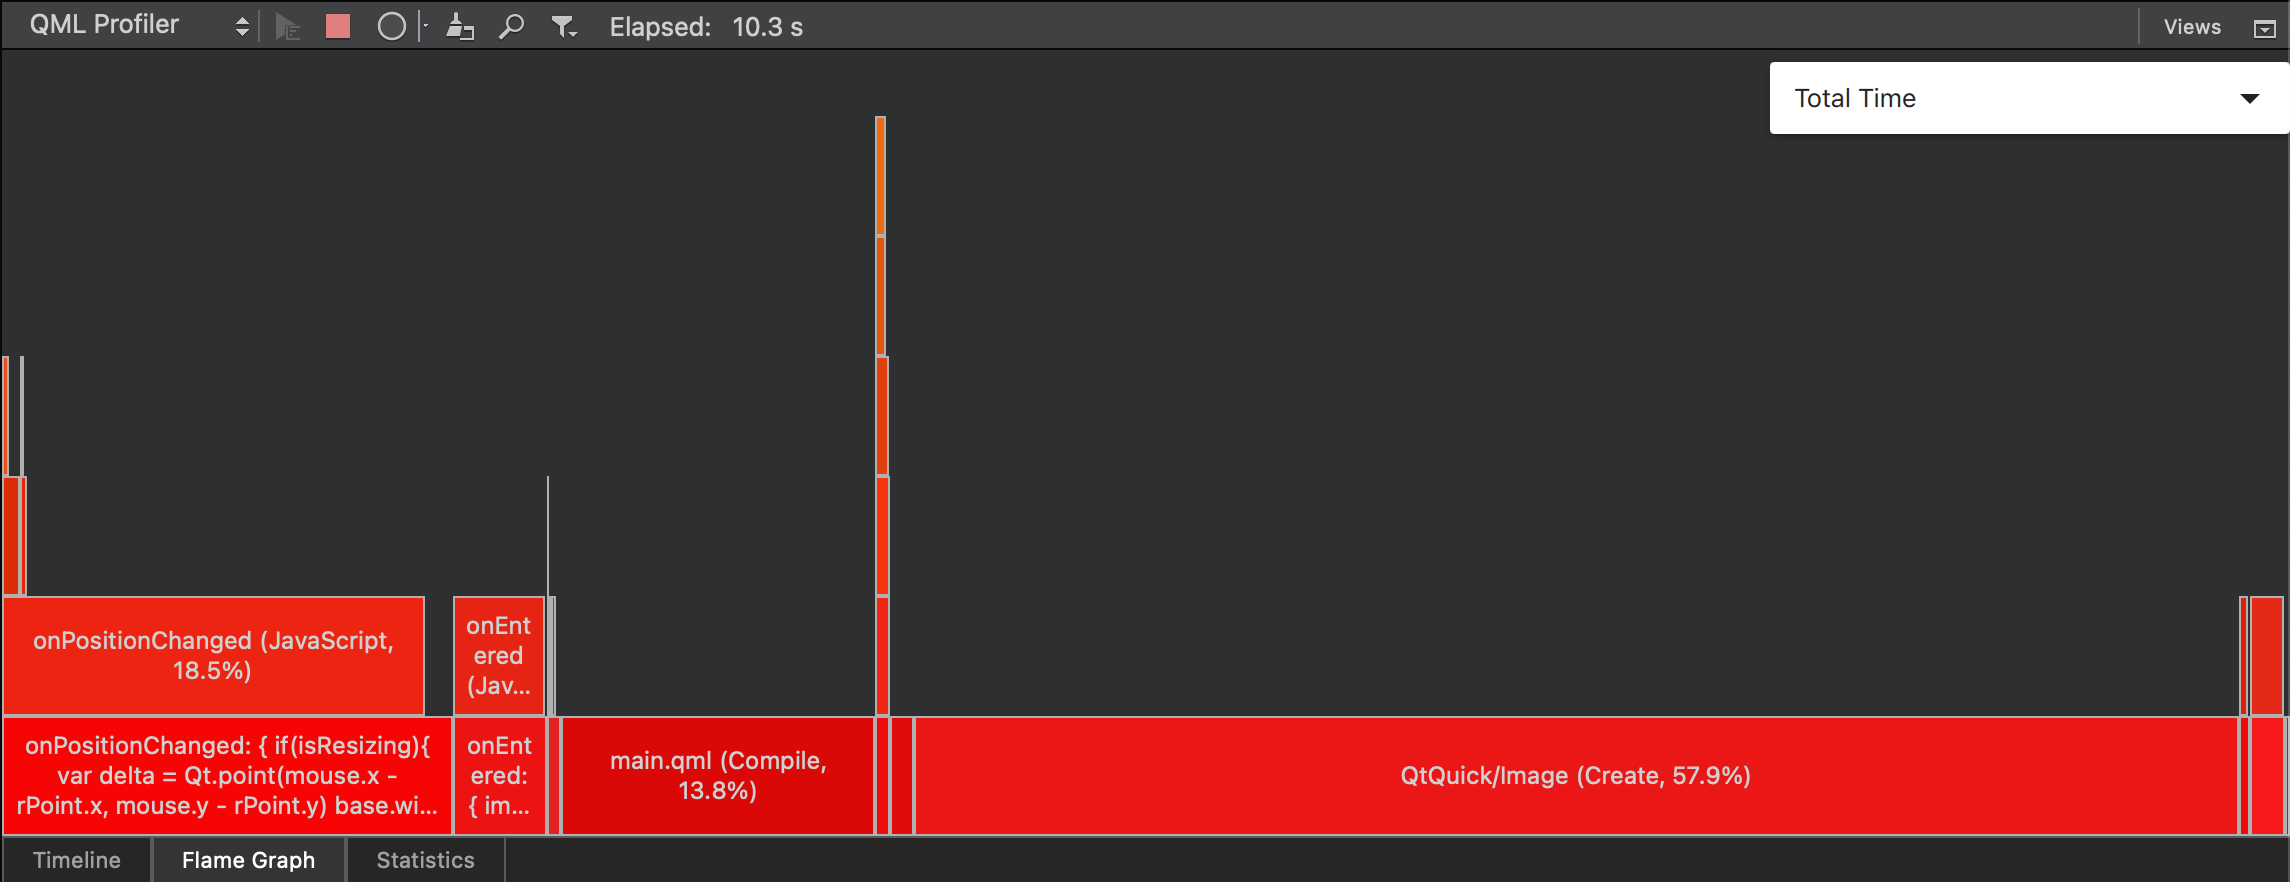
\includegraphics[scale=0.30]{qml-prof-05.png}
\end{center}
\caption{Flame Graph - Total Time}
\label{fig: qml-05}
\end{figure}

Rezultat analize prikazan kroz Flame Graph, za sekciju memorijskog utroška izgleda ovako \ref{fig: qml-06}.

\begin{figure}[h!]
\begin{center}
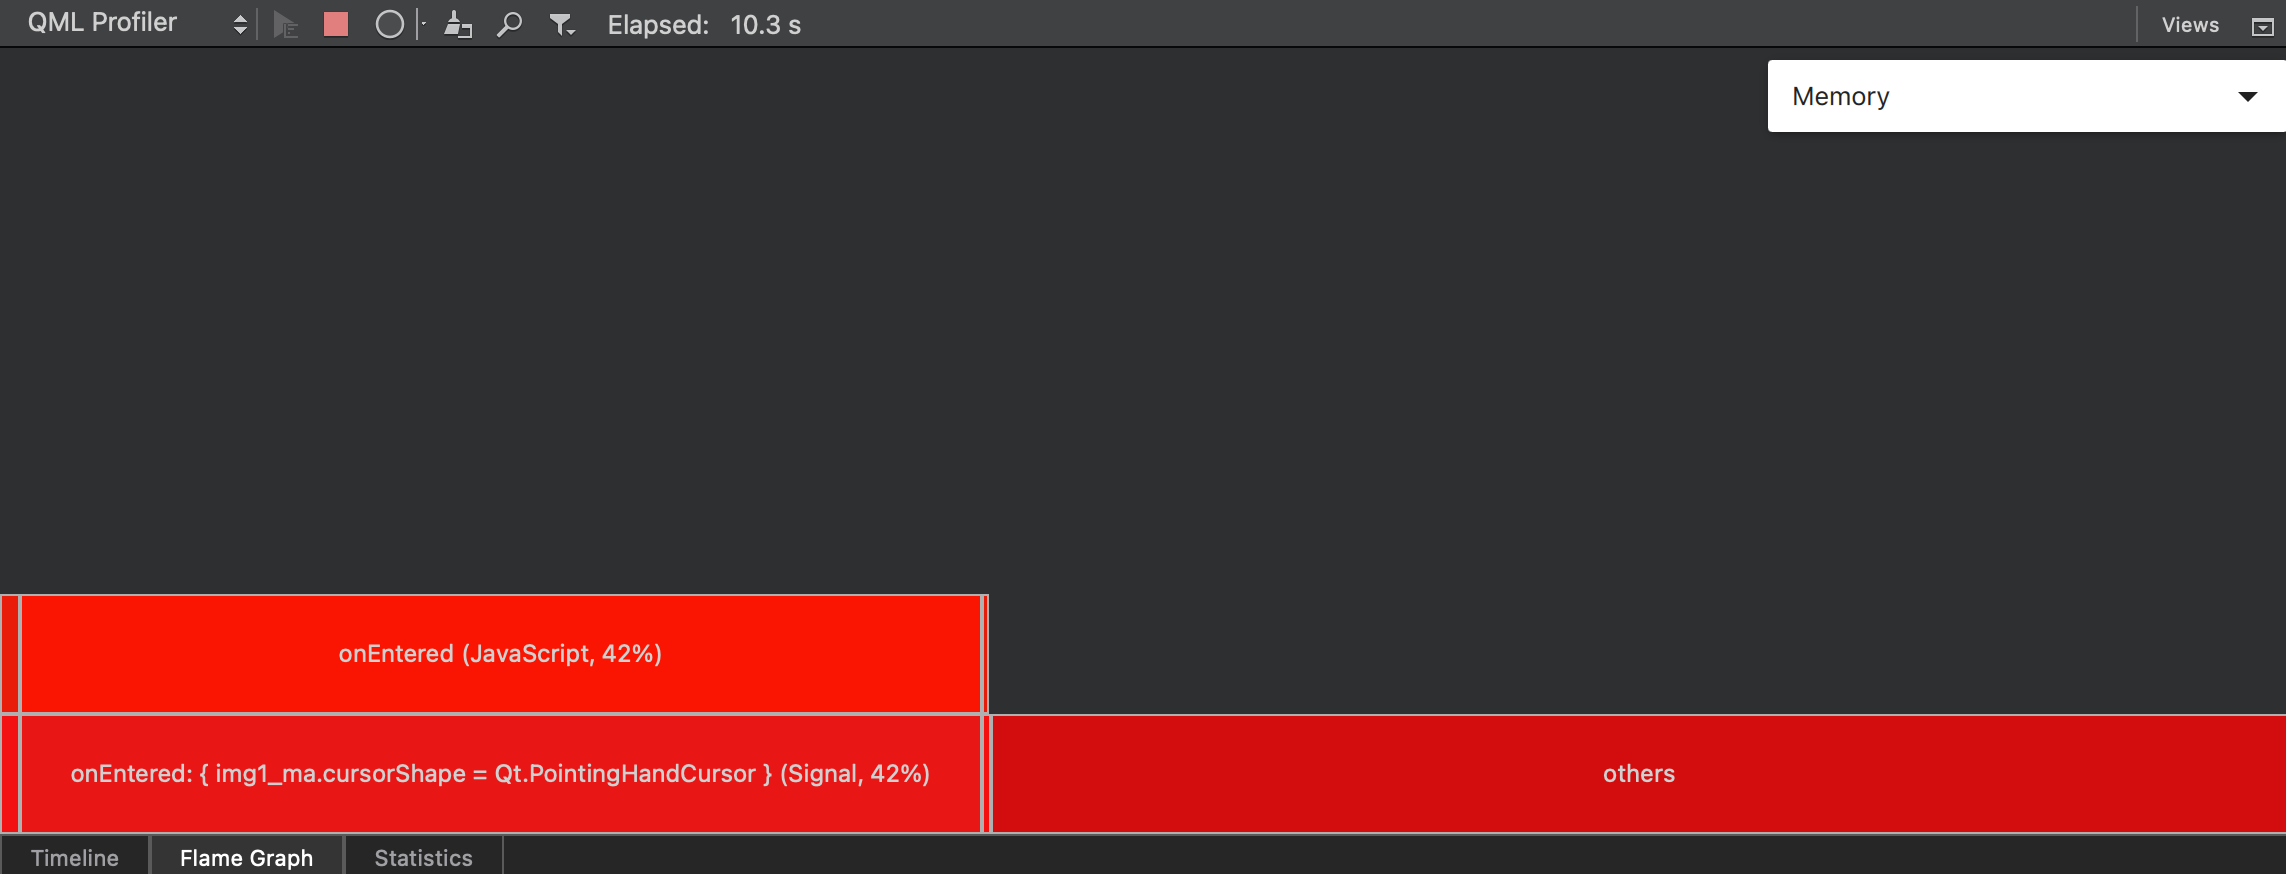
\includegraphics[scale=0.30]{qml-prof-06.png}
\end{center}
\caption{Flame Graph - Memory}
\label{fig: qml-06}
\end{figure}

Rezultat analize prikazan kroz Flame Graph, za sekciju alokacija memorije izgleda ovako \ref{fig: qml-07}.

\begin{figure}[h!]
\begin{center}
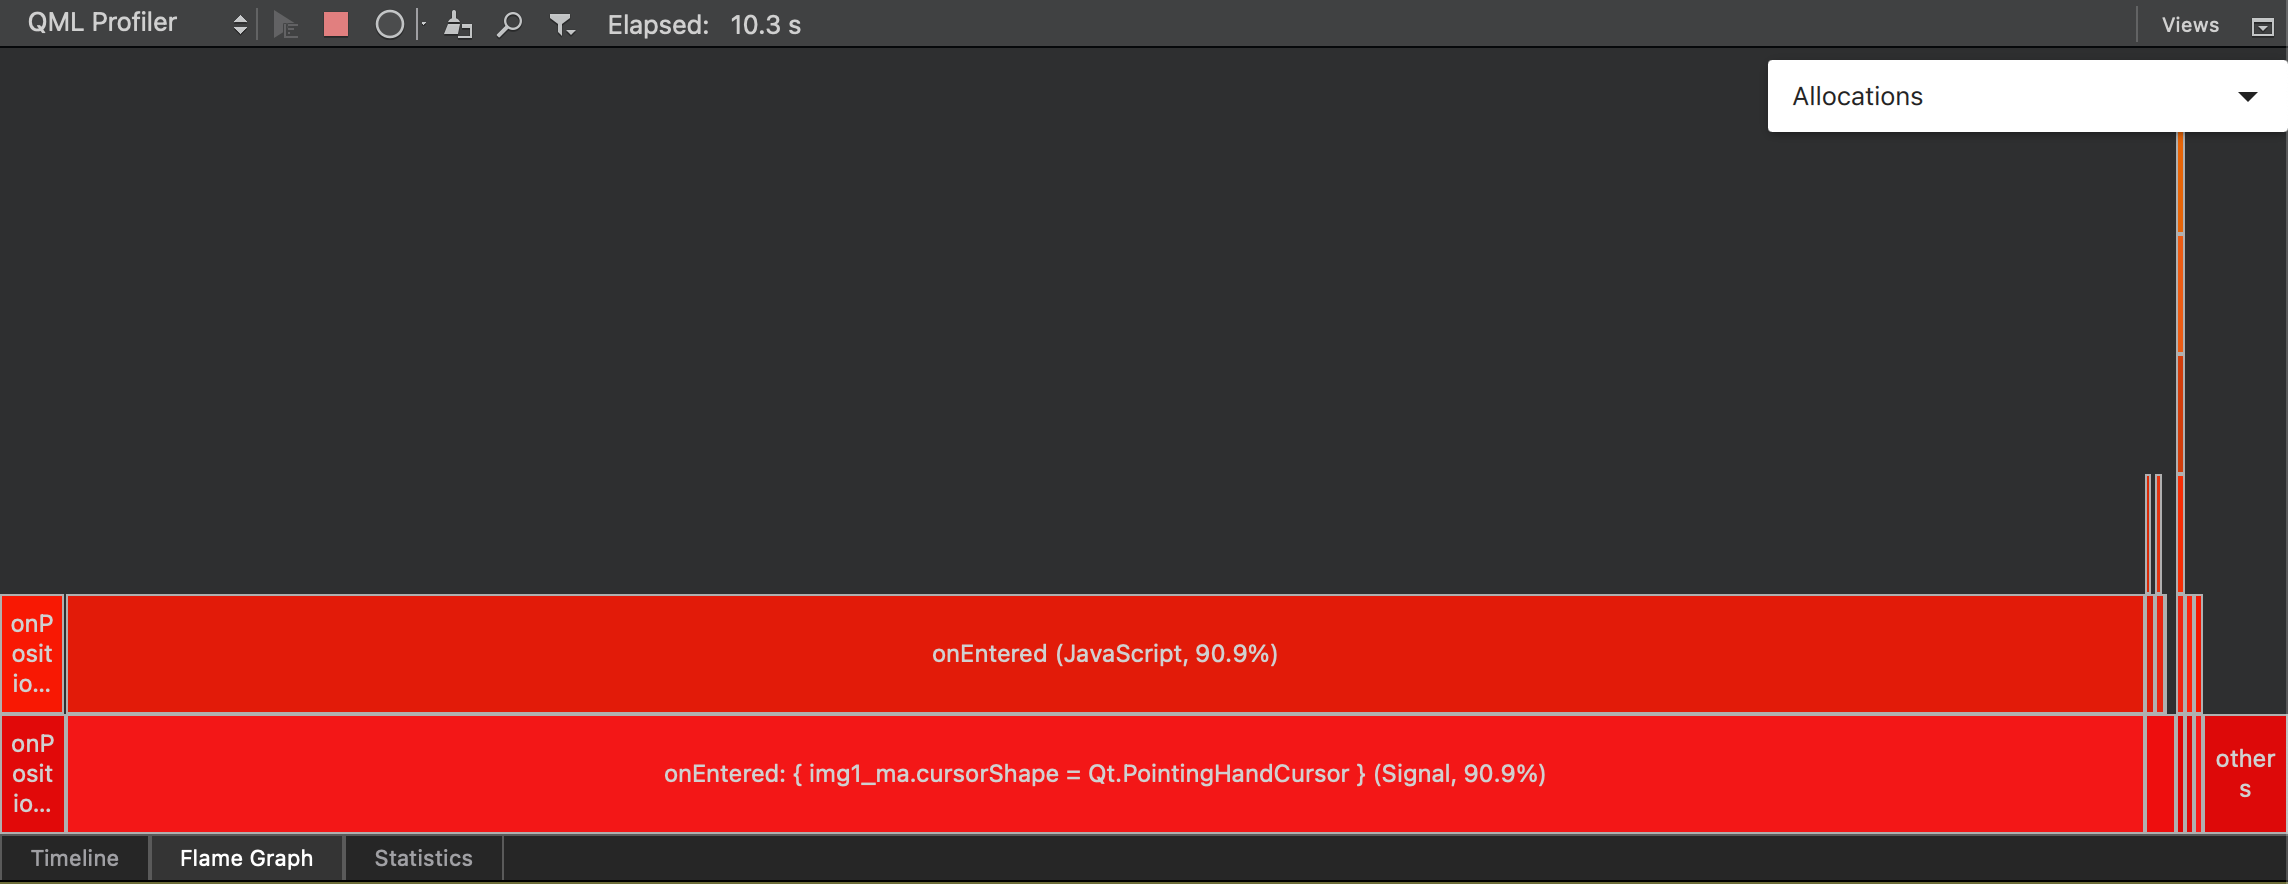
\includegraphics[scale=0.30]{qml-prof-07.png}
\end{center}
\caption{Flame Graph - Allocations}
\label{fig: qml-07}
\end{figure}

Na kraju se može videti statistički prikaz analize nad svim komponentama ove aplikacije \ref{fig: qml-08}.

\begin{figure}[h!]
\begin{center}
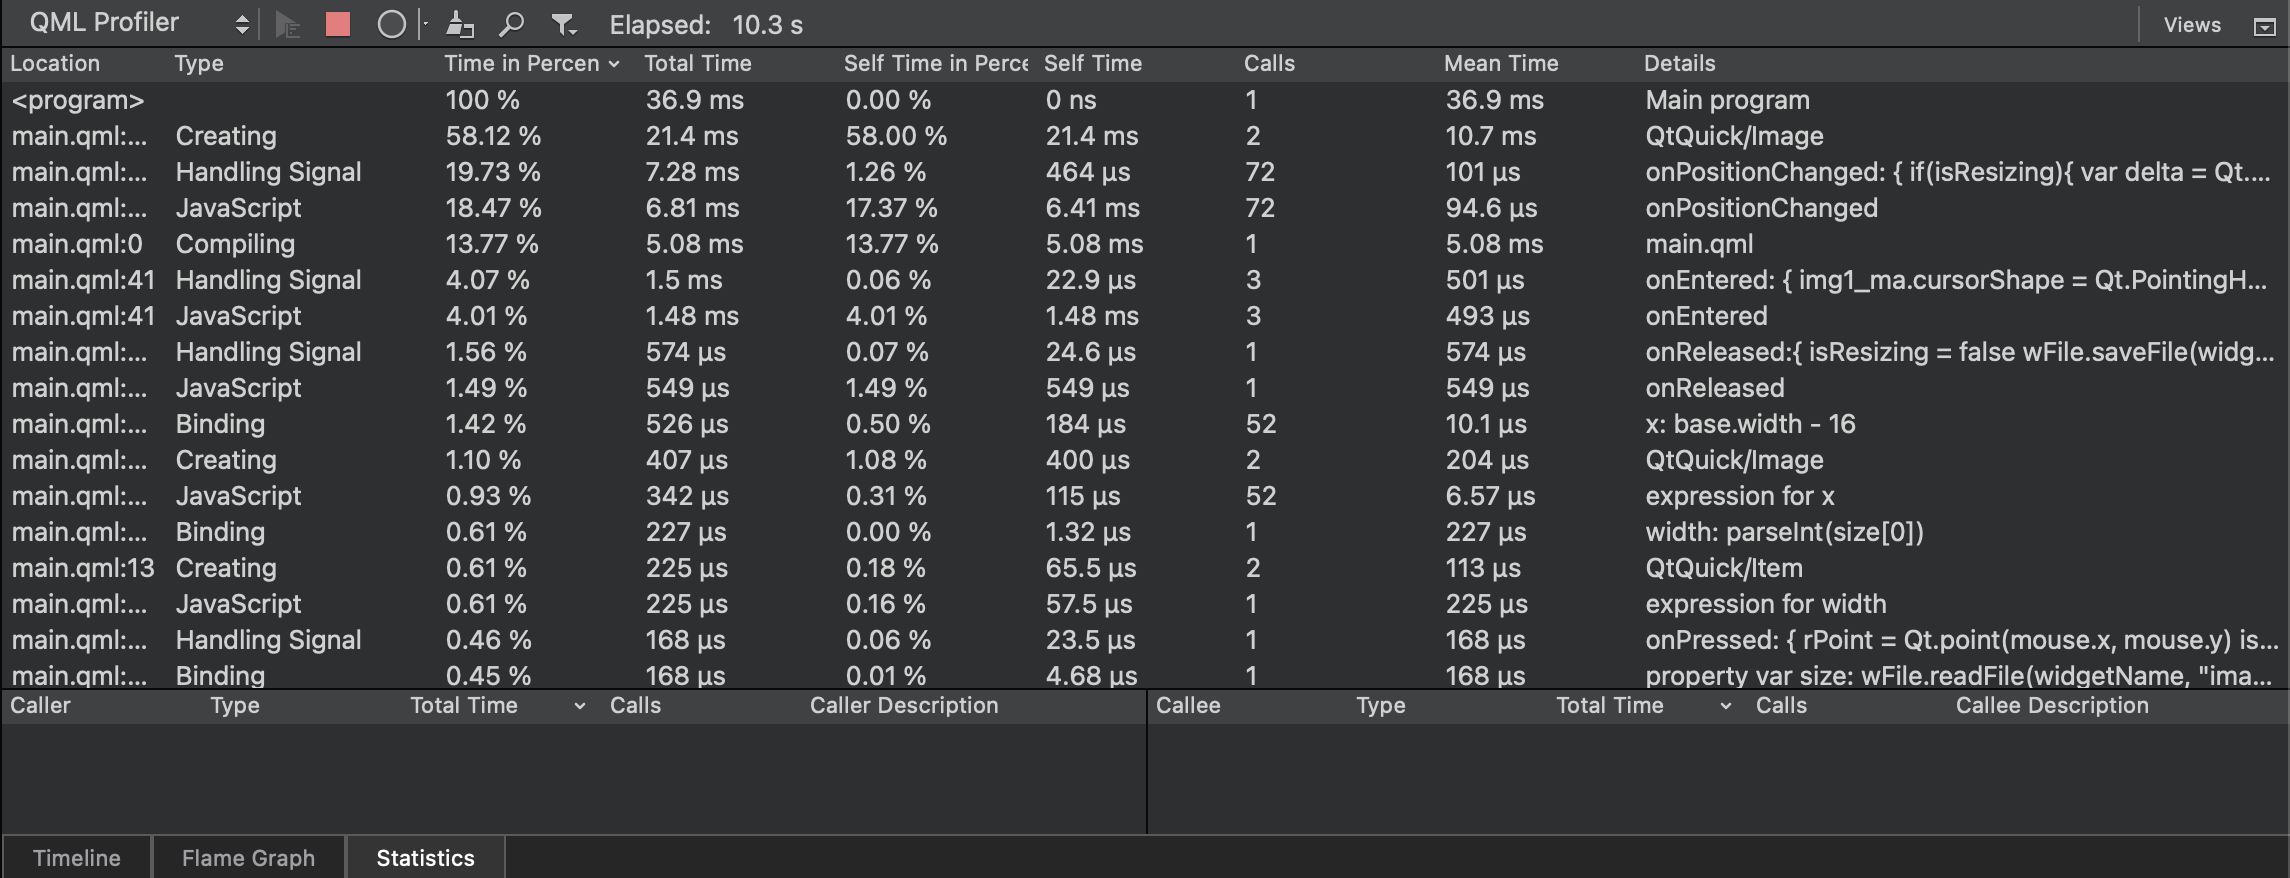
\includegraphics[scale=0.30]{qml-prof-08.png}
\end{center}
\caption{Statistics}
\label{fig: qml-08}
\end{figure}

Na osnovu ovih dijagrama možemo videti performanse aplikacije tokom izvršavanja i zahvaljujući njima odrediti koji delovi koda troše najviše vremena i memorije i na osnovu toga ih optimizovati.

U okviru rezultata ovog alata nad analiziranim projektom nisam primetio problem sa performansama tokom izvršavanja aplikacije.

\end{document}
